\section{Evaluation}

Our experimental setup consists of 4 machines each with two sockets
equipped Intel Xeon E5-2640 CPU's and 265GB of main memory evenly
spread across two NUMA domains. Each machine has a Mellanox ConnectX-5
100Gbps NIC installed in a 16x PCIe slot. Each server is
interconnected via a 100Gbps Mellanox Onyx Switch. We designate a
single server to run as both the memory server (MS) and as the meta
data server (DN). Two machines are configured as clients, and a single
machine acts as a programmable switch.

All clover servers are configured using default routing settings.
Clients are configured to send directly to metadata and data servers.
We install OpenFlow rules on our Mellanox Onyx switch to redirect all
traffic to our DPDK packet switch.

\subsection{Conflict Resolution}

We test the performance gains of resolving write conflicts using our
middlebox solution. Clover clients are configured to run a YCSB-A
benchmark, 50\% read, 50\% write for 1 million requests. Request for
keys are distributed based on a zipf distribution generated with an
\textit{s} value of 0.75.\todo{show exactly what this means}. In each
experiment the number of client threads is increased which in turn
increases the load on the system. Clover request are blocking, and
thus the throughput is a factor of both the request latency and the
number of client threads. Figure~\ref{fig:throughput} shows the
performance gains by resolving write conflicts in flight.

As the number of clients increases so to does the probability that two
client threads will make concurrent writes to the same key. The number
of conflicts resolved in flight directly correlates to throughput
improvements as each successful request reduces the multiple round
trips necessary to resolve write conflicts. Our current implementation
provides a 1.42x throughput improvement at 64 client threads.

Our current experiments are limited by the scale of our experimental
setup, i.e more client machines can produce higher throughputs.
\todo{This is the speculation part we should cut}. 
The number of in flight conflicts is also effected by the zipf
distribution. We use a zipf of 0.75, however a zipf of 1.0 would
result in a distribution skewed towards fewer keys, which in turn
would result in higher conflicts. We found that Clovers current design
leads to high contention on ConnectX-5 NIC's as the number of RDMA
compare and swaps to the same memory region across different queue
pairs increases~\cite{design-guidelines}. In future work we plan to
both scale up the number of our client threads. Additionally our
design reduces the need for expensive compare and swap operations as
all cached keys have no conflicts. Our future implementations will
seek to reduce or eliminate c\&s and replace them with low overhead
RDMA writes.

\begin{figure}
    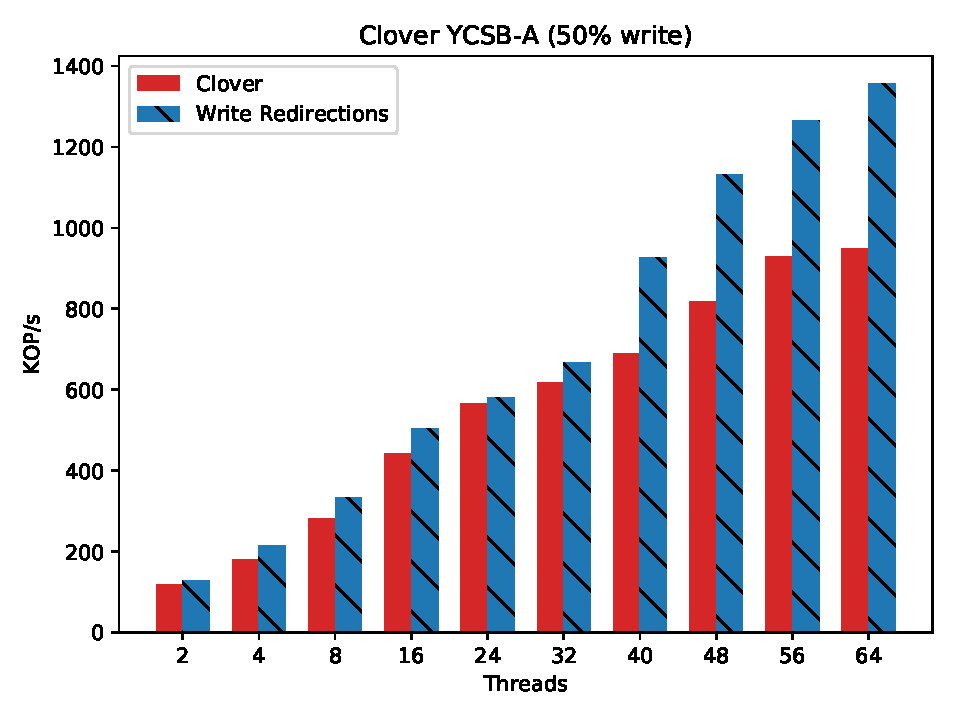
\includegraphics[width=0.45\textwidth]{fig/throughput.pdf}
    \caption{Default Clover throughput vs Clover with write conflict
    detection and correction turned on.}
    \label{fig:throughput}
\end{figure}

\subsection{Memory Consumption}

Resources on networking hardware is scarce. High end SoC SmartNIC's
have just a few GB of RAM, and programmable switches have only MB's of
SRAM. Moreover the use of this memory is not free. Using memory for
any purpose other than buffer packets has a direct performance cost as
the number of packets which can be successfully buffered drops. Our
design takes the preciousness of memory in network into account. The
metadata we cache in network in the minimal necessary to resolve write
conflicts. While Clover's meta data consists of many MB of garbage
collection and version data we only cache the virtual address of the
last write per key. In addition we track the last key written per
client thread. Clients are not explicitly known to our middlebox and
are identified at runtime by their QP. Tracking clients in this way is
necessary to detect write conflicts in clover. This overhead could be
eliminated by explicitly adding key information to c\&s requests.

Figure~\ref{fig:memory} Shows the memory overhead as a function of
keys. Note that 100K keys can be supported using 7\% of the available
memory on a Barefoot Tofino programmable switch (22MB).

\begin{figure}
    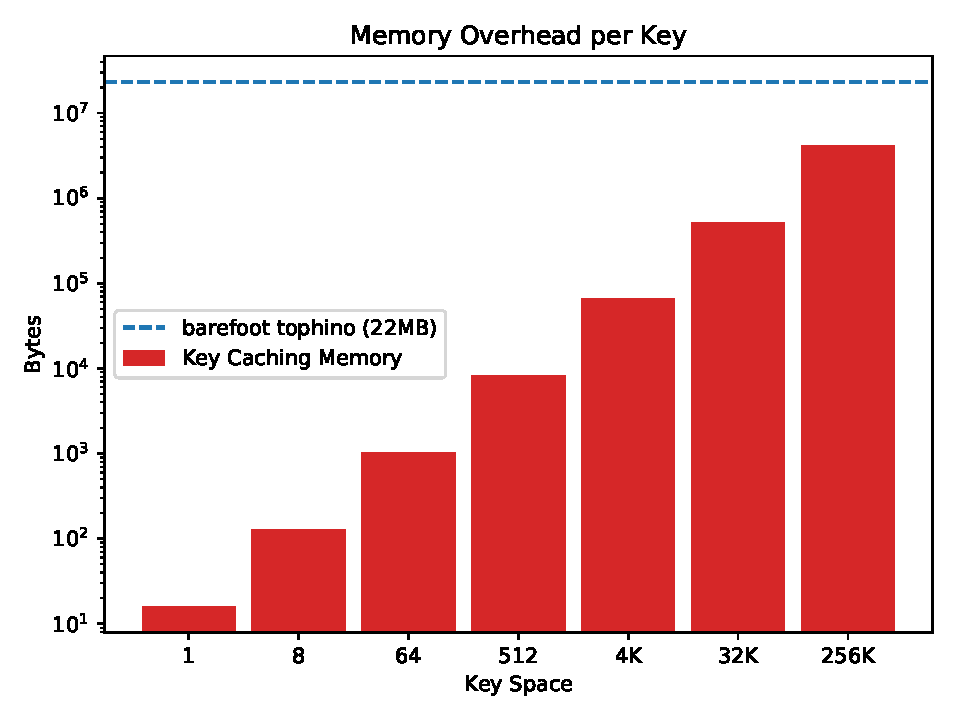
\includegraphics[width=0.45\textwidth]{fig/memory.pdf}
    \caption{Cost of caching metadata in network vs keyspace size.}
    \label{fig:memory}
\end{figure}

\subsection{Caching top \textit{N} keys} 
%%
Hot keys which are written frequently are the most likely to
contribute to conflict. Caching only hot keys results in relatively
large performance gains while requiring only a small portion of the
memory required to cache the entire keyspace. We test the effect of
caching only hot keys by restricting our in network cache to track and
resolve conflicts on only the top \textit{N} keys. In this experiment
RDMA requests for keys which are not caches pass through our middlebox
without modification, conflicts are resolved using Clovers
reconciliation protocol. We ran our experiment with 64 client threads,
with a total keyspace size of 1024 keys. Figure~\ref{fig:cache} shows
the relative throughput gains from caching the top N keys. The request
distribution is zipf(0.75), therefore the vast majority of conflicts
occur on the top 8 keys. The in network memory requirement for 8 keys
is 128 Bytes, which results in 1.3x throughput improvement.

\begin{figure}
    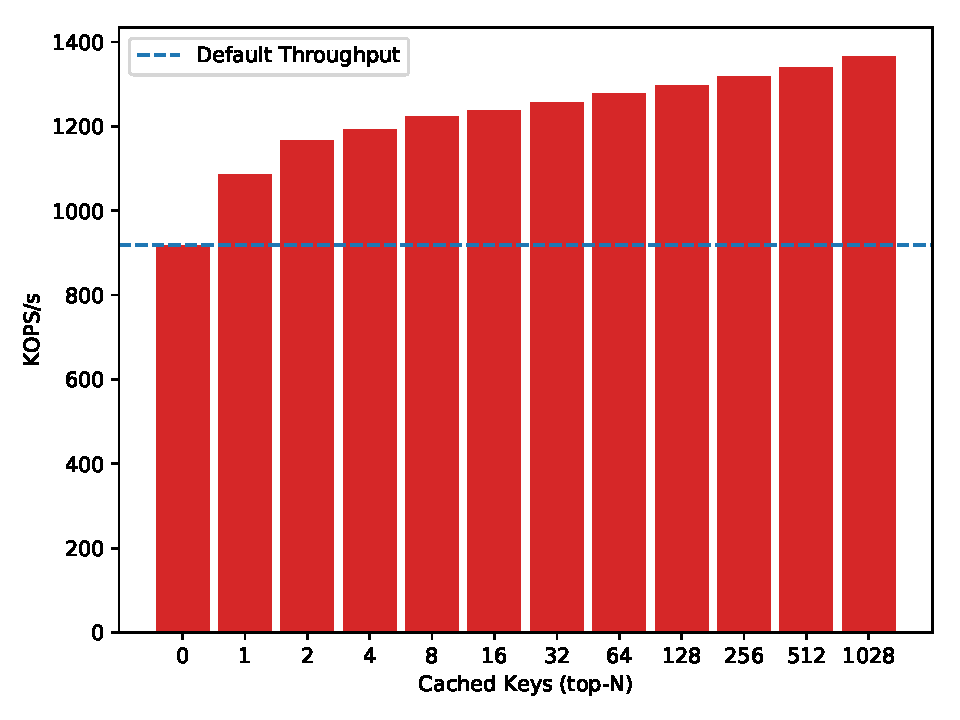
\includegraphics[width=0.45\textwidth]{fig/cache.pdf}
    \caption{Performance as a function of keys cached. Caching a few
    of the top n keys provides the greatest marginal throughput
    benefits.}
    \label{fig:cache}
\end{figure}

